
    \documentclass{standalone}
\usepackage{tkz-fct}
\usepackage{tkz-euclide}
\usepackage{color}
\renewcommand*\familydefault{\sfdefault}
\usepackage{sansmath}
\usepackage{amsmath}
\sansmath
\definecolor{gray75}{gray}{0.75}
\begin{document}
 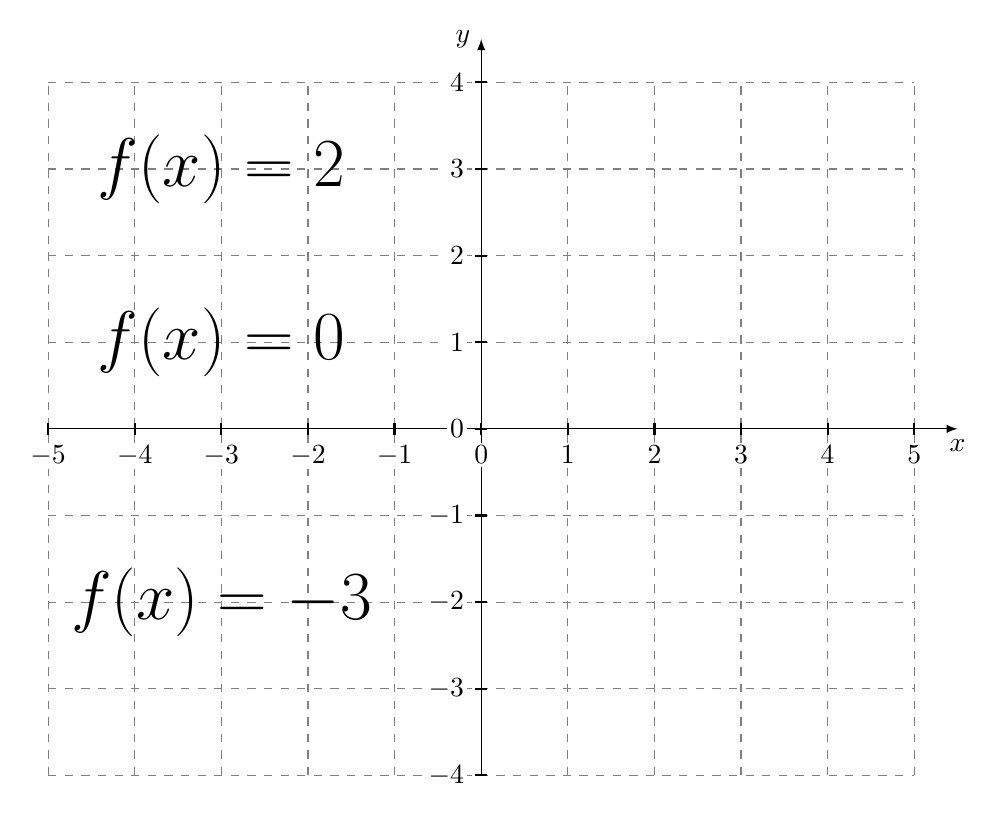
\begin{tikzpicture}[scale=1.1]
   \tkzInit[xmax=5.0,ymax=4.0,xmin=-5.0 ,ymin=-4.0]
   \begin{scope}[dashed]
     \tkzGrid
   \end{scope}
   \tkzDrawX[label={$x$}]
   \tkzDrawY[label={$y$}]
   \tkzLabelX
   \tkzLabelY
   \tkzFct[line width=2pt,domain=-5:5]{(2)}
   \tkzFct[line width=2pt,domain=-5:5]{(0)}
   \tkzFct[line width=2pt,domain=-5:5]{(-3)}
   \tkzText(-3,3){\Huge$f(x)=2$}
   \tkzText(-3,1){\Huge$f(x)=0$}
   \tkzText(-3,-2){\Huge$f(x)=-3$}
\end{tikzpicture}
\end{document}
